\documentclass{standalone}
\usepackage{graphicx}	
\usepackage{amssymb, amsmath}
\usepackage{color}

\usepackage{tikz}
\usetikzlibrary{calc, math}
\usepackage{pgfmath}

\definecolor{light}{RGB}{220, 188, 188}
\definecolor{mid}{RGB}{185, 124, 124}
\definecolor{dark}{RGB}{143, 39, 39}
\definecolor{highlight}{RGB}{180, 31, 180}
\definecolor{lightteal}{RGB}{186, 219, 219}
\definecolor{midteal}{RGB}{124, 186, 186}
\definecolor{darkteal}{RGB}{38, 142, 142}
\definecolor{darkerteal}{RGB}{0, 124, 124}
\definecolor{gray10}{gray}{0.1}
\definecolor{gray20}{gray}{0.2}
\definecolor{gray30}{gray}{0.3}
\definecolor{gray40}{gray}{0.4}
\definecolor{gray60}{gray}{0.6}
\definecolor{gray70}{gray}{0.7}
\definecolor{gray80}{gray}{0.8}
\definecolor{gray90}{gray}{0.9}
\definecolor{gray95}{gray}{0.95}

% #1: x0
% #2: y0
% #3: Rx
% #3: Ry
\newcommand{\randpoints}[4]{
  ({#1 + (1 + 0.2 * rand) * #3 * (-1)},      {#2 + (1 + 0.2 * rand) * #4 * (0)})
  ({#1 + (1 + 0.2 * rand) * #3 * (-0.7071)}, {#2 + (1 + 0.2 * rand) * #4 * (+0.7071)})
  ({#1 + (1 + 0.2 * rand) * #3 * (0)},       {#2 + (1 + 0.2 * rand) * #4 * (+1)})
  ({#1 + (1 + 0.2 * rand) * #3 * (+0.7071)}, {#2 + (1 + 0.2 * rand) * #4 * (+0.7071)})
  ({#1 + (1 + 0.2 * rand) * #3 * (+1)},      {#2 + (1 + 0.2 * rand) * #4 * (0)})
  ({#1 + (1 + 0.2 * rand) * #3 * (+0.7071)}, {#2 + (1 + 0.2 * rand) * #4 * (-0.7071)})
  ({#1 + (1 + 0.2 * rand) * #3 * (0)},       {#2 + (1 + 0.2 * rand) * #4 * (-1)})
  ({#1 + (1 + 0.2 * rand) * #3 * (-0.7071)}, {#2 + (1 + 0.2 * rand) * #4 * (-0.7071)})
}

\begin{document}

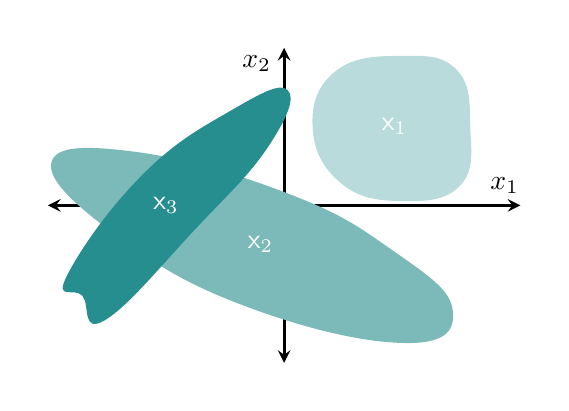
\begin{tikzpicture}[scale=1.0]

  \pgfmathsetseed{1}

  \pgfmathsetmacro{\ys}{3.95};

  \draw[white] (-3.25, -2.25) rectangle (3.25, 2.25);
  
  \draw [<->, >=stealth, line width=1] (0, -2) -- +(0, 4);
  \draw [<->, >=stealth, line width=1] (-3, 0) -- +(6, 0);
  
  \node at (2.8, 0.25) { $x_{1}$ };
  \node at (-0.35, 1.8) { $x_{2}$ };
  

  \fill[lightteal]
    plot [smooth cycle, tension=0.75] coordinates { \randpoints{1.5}{1}{1}{1} } -- cycle;
  \node[white] at (1.4, 1) { $\mathsf{x}_{1}$ };

  \fill[midteal, rotate=-20]
    plot [smooth cycle, tension=0.75] coordinates { \randpoints{0}{-0.5}{2.5}{0.75} } -- cycle;
  \node[white] at (-0.3, -0.5) { $\mathsf{x}_{2}$ };
  
  \fill[darkteal, rotate=-45]
    plot [smooth cycle, tension=0.75] coordinates { \randpoints{-1}{-1}{0.5}{2} } -- cycle;
  \node[white] at (-1.5, 0) { $\mathsf{x}_{3}$ };
  
\end{tikzpicture}

\end{document}  